\documentclass[a4paper]{article}

\usepackage[english]{babel}
\usepackage[utf8]{inputenc}
\usepackage{amsmath}
\usepackage{graphicx}
\usepackage[colorinlistoftodos]{todonotes}

\title{QF603 Group Mini-Project 1}

\author{Group F}

\date{\today}

\begin{document}
\maketitle

\begin{abstract}
Enter a sh ort summary here. What topic do you want to investigate and why? What experiment did you perform? What were your main results and conclusion?
\end{abstract} 

\section{Task 1}
\label{sec:introduction}

\subsection{Verification of Dow Jones index}
\begin{flushleft}
The summation of the 30 component stock prices : 3742.98 \linebreak 
DJIA index value :
$$ DJIA index = \frac{3742.98}{0.14748071991788} = 25379.453002969884
$$
\end{flushleft}

\subsection{Findings about S\&P 500}
The popular S\&P 500, known in full as the Standard \& Poor’s 500, once took humbler forms. First called “The Composite Index”, the initial form of the S\&P 500 tracked only a handful of stocks when Poor’s Publishing introduced it in 1923. The index saw its number of tracked stocks increase to 90 in 1926, and in 1941, Poor’s Publishing merged with Standard Statistics to form Standard \& Poor’s Corporation. It was only until 4 March 1957 that the index saw its number of tracked stocks increase to 500 and its name changed to the “S\&P 500” that we are all more familiar with in recent years. Only a handful of the S\&P 500’s original members, such as Coca-Cola, Pfizer and PepsiCo are still in the index today.

Unlike the older Dow Jones Industrial Average (also known as “the Dow”), which assigns index component weights by price, the S\&P 500 weighs its components by market capitalisation. It is for this reason, amongst many others, that the S\&P 500 is sometimes regarded as more representative of the U.S. equity market. The S\&P 500’s superior breadth (the S\&P 500 tracks 505 stocks, the Dow’s tracks 30) and depth (the S\&P 500 reflects stocks making up \% of the U.S. equity market, compared to the Dow’s \%) of coverage compared to the Dow’s are often also other pull factors for institutional investors. It is also noteworthy that all of the Dow’s 30 components are also included in the S\&P 500, so investors seeking a broader version of Dow may consider the S\&P 500 as one of their viable options.

The S\&P 500’s price is computed by simply dividing the sum of the weighted prices of its components by a divisor, which is adjusted in the event of stock splits, spinoffs or any other event which may unduly and numerically alter the component stock’s price. Components of the S\&P 500 have to undergo a selection process by a committee before being included in the index.  When being considered for inclusion into the S\&P 500, a stock is assessed on nine different criteria, with domicile, exchange listing, organisational structure \& share type, market capitalisation and liquidity just being just a few of said criteria. Usually, only large cap and heavily traded stocks make it into the S\&P 500.


\subsection{Time series of the two indexes}

\begin{figure}[h]
	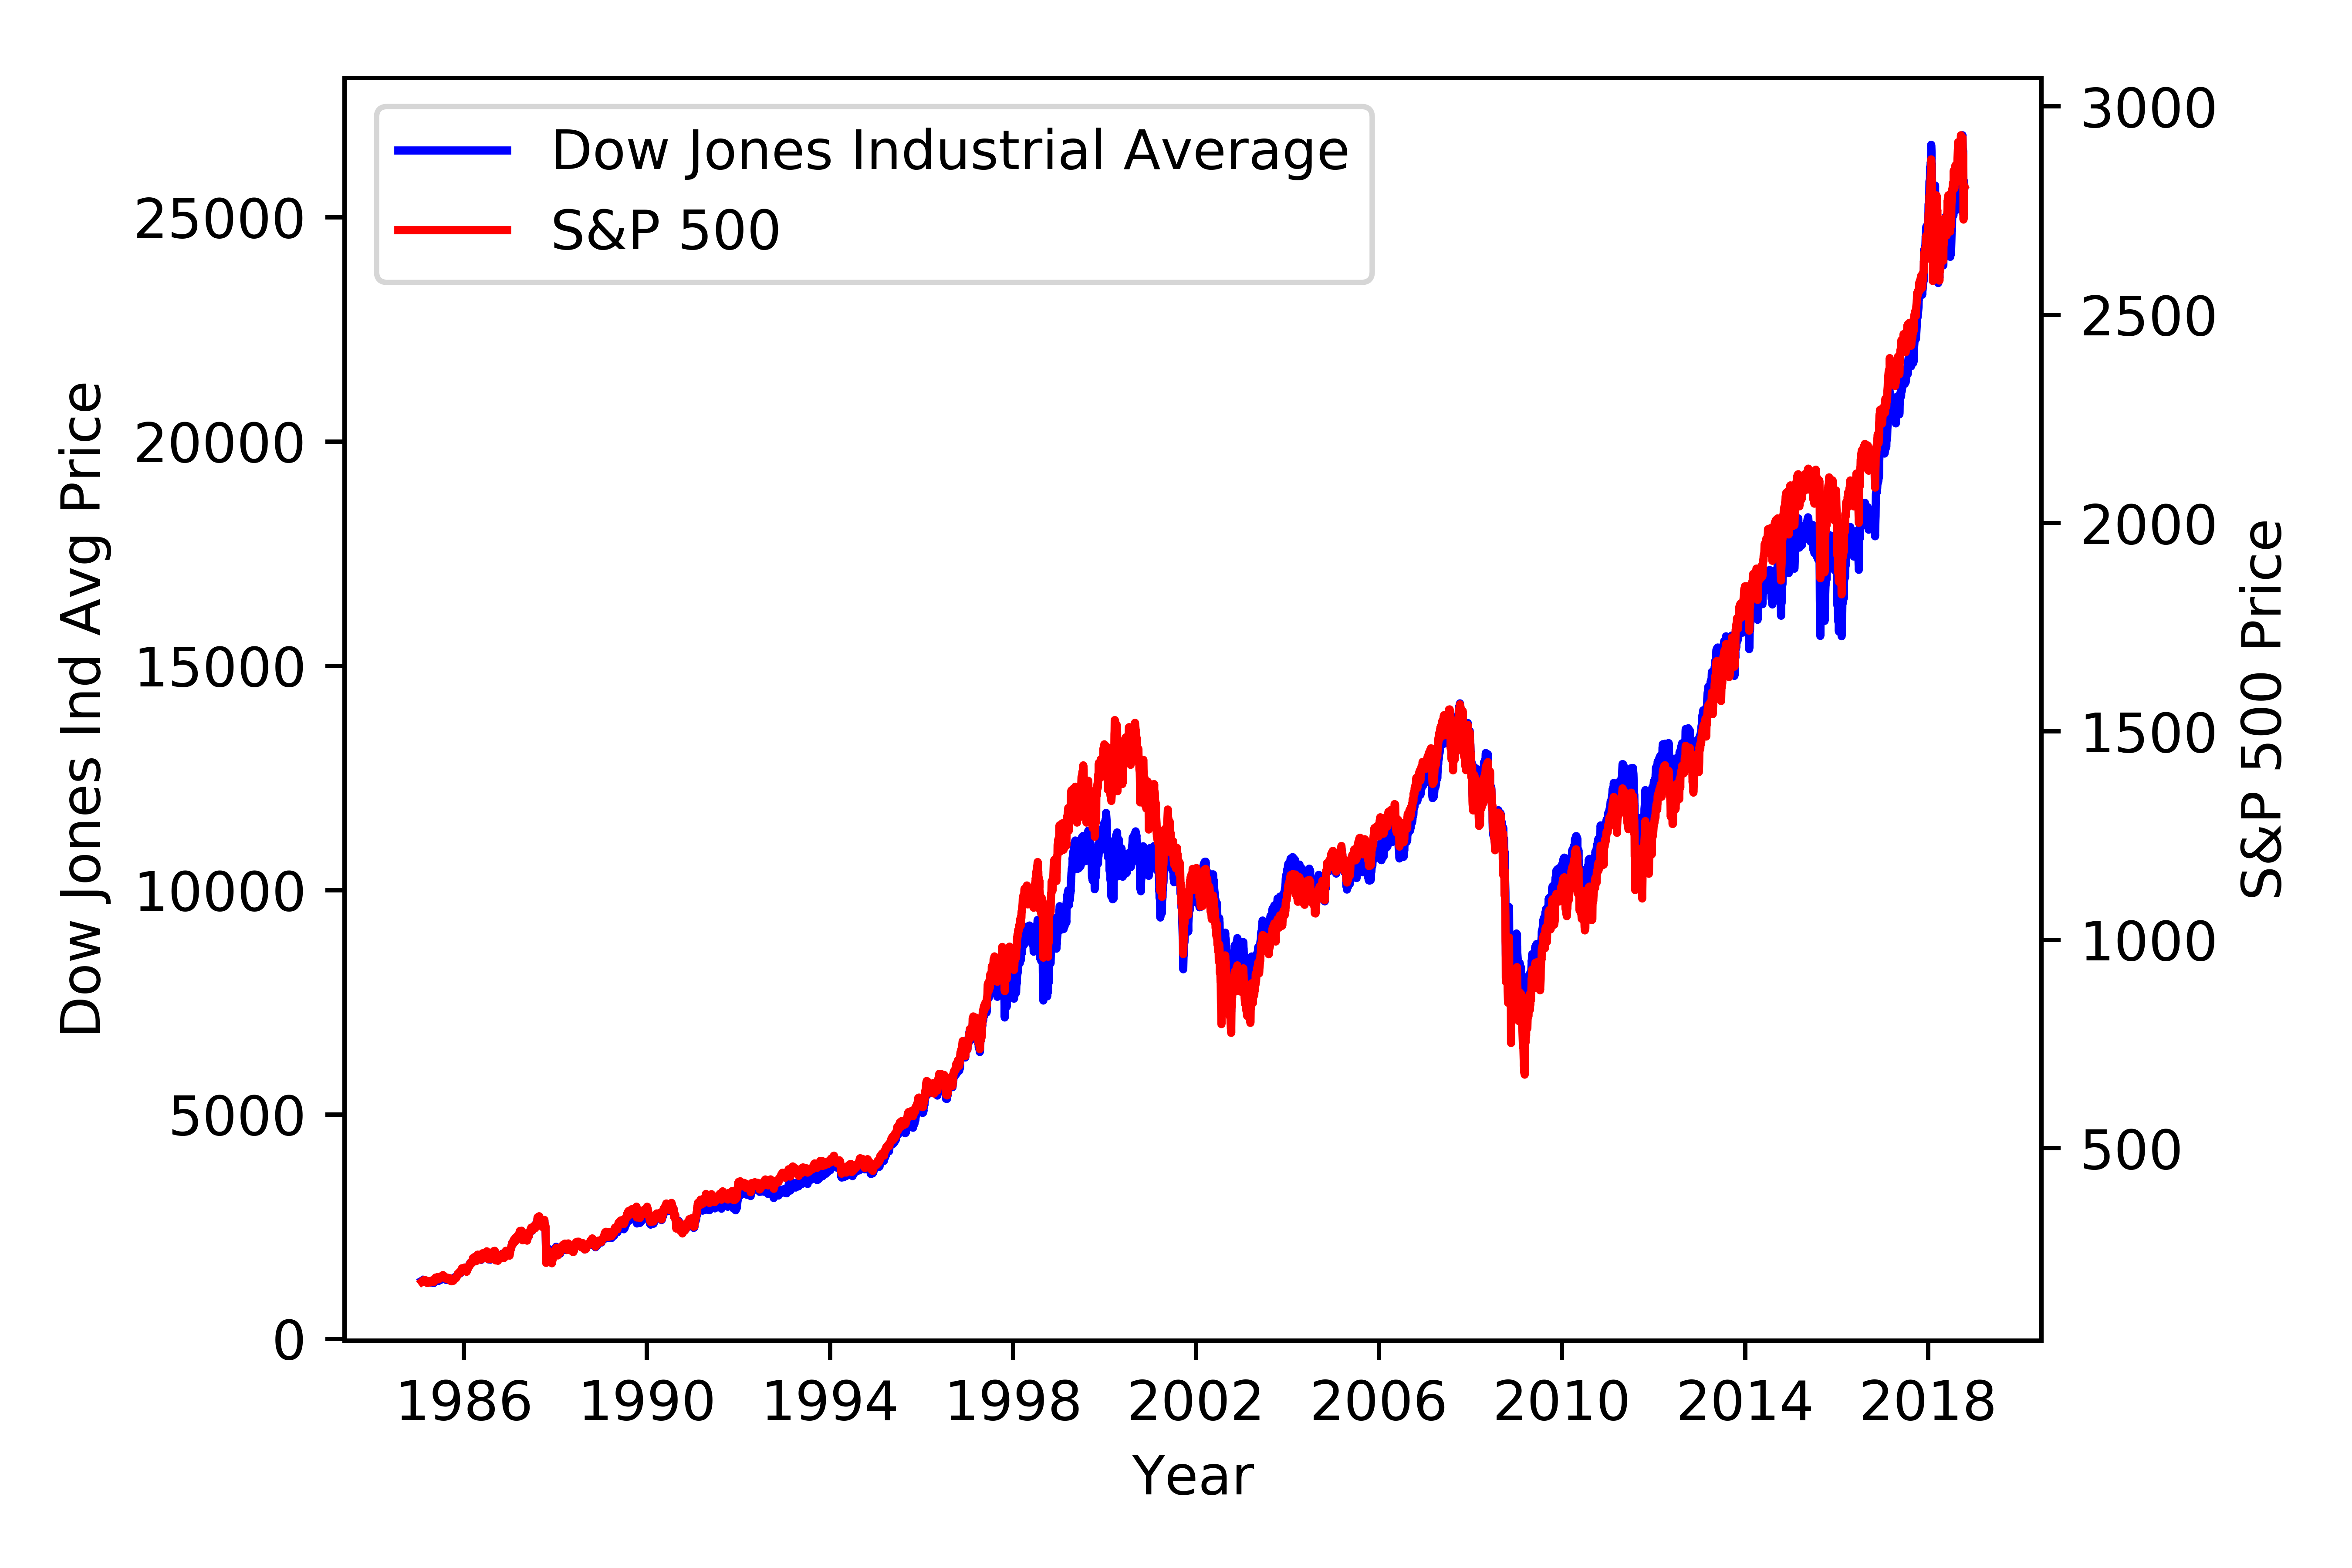
\includegraphics[width=\linewidth]{time_series.png}
	\caption{Time series of Dow Jones and S\%P 500 indexes}
\end{figure}

\subsection{Time series of log returns}

\newpage
%\pagebreak
\subsection{Chart of daily log returns}

\begin{figure}[h!]
	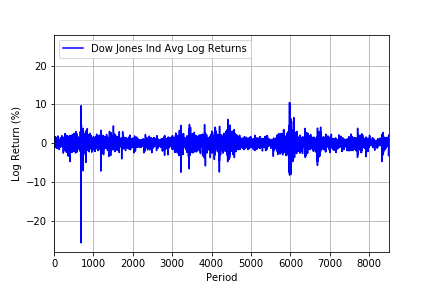
\includegraphics[width=\linewidth]{DJI_logret.png}
	\caption{Time series of Dow Jones Index log return}
\end{figure}
\begin{figure}[h!]
	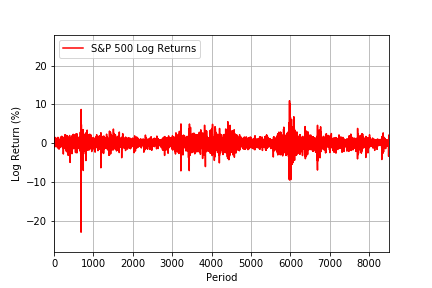
\includegraphics[width=\linewidth]{SP_logret.png}
	\caption{Time series of S\%P 500 log return}
\end{figure}

\subsection{Sample mean and sample variance of log return}
\begin{flushleft}
Sample mean of Dow Jones Index : 0.000351774083023244  \linebreak 
Sample mean of S\&P 500 Index : 0.0003237962025912197  \linebreak 
Sample variance of Dow Jones Index : 0.00012082440895848629  \linebreak 
Sample variance of S\&P 500 Index : 0.00012653731363052728  \linebreak 
\end{flushleft}

\subsection{Annualized average and volatility of log return}
\begin{flushleft}
Annualized log return of Dow Jones Index : 0.08864706892185749 \linebreak 
Annualized log return of S\&P Index : 0.08159664305298736 \linebreak 
Annualized volatility of Dow Jones Index : 0.17449283955950326 \linebreak 
Annualized volatility of S\&P Index : 0.17857044278069334 \linebreak 
\end{flushleft}

\subsection{Sample skewness and sample kurtosis}
\begin{flushleft}
	Skewedness of Dow Jones Index : -1.6915630820777834 \linebreak 
	Skewedness of S\&P 500 : -1.283239589463856 \linebreak 
	Kurtosis of Dow Jones Index : 45.39466619559327 \linebreak 
	Kurtosis of S\&P 500 : 31.44364518517353 \linebreak 
\end{flushleft}

\subsection{Jarque-Bera test statistics}
\begin{flushleft}
Jarque-Beta Statistic of Dow Jones Ind Avg's Returns: 633852.49\linebreak
Jarque-Beta Statistic of S\&P 500's Returns: 285696.06\linebreak

Critical Chi-Square Value with 2 Degrees of Freedom: 5.991465\linebreak

Thus, we are able to reject null hypothesis that JB=0 for both indices.\linebreak
\end{flushleft}

\section{Task2}

\subsection{Correlation bewteen log returns of Dow Jones Index and S\&P500}
\begin{flushleft}
Correlation: 0.965149
\end{flushleft}

\subsection{Two-sample t-test of the two indexes}
\begin{flushleft}
t Statistic: 0.164005

Critical t Values: +/-1.960104

Thus, we are unable to reject null hypothesis that mean differences are 0.
\end{flushleft}

\subsection{F-test of the two indexes}
\begin{flushleft}
F Statistic: 1.047283

Critical F Values: 0.958368, 1.04344

Thus, we are able to reject null hypothesis that the 2 population variances are equal.
\end{flushleft}

\newpage
\begin{thebibliography}{9}
\bibitem{nano3}
  K. Grove-Rasmussen og Jesper Nygård,
  \emph{Kvantefænomener i Nanosystemer}.
  Niels Bohr Institute \& Nano-Science Center, Københavns Universitet

\end{thebibliography}
\end{document}